\chapter{Конструкторская часть}

\section{Нерекурсивный алгоритм}

Схема алгоритма приведена на рисунке~\ref{fig:shemanum1}.  

\begin{figure}[h!]
	\centering
	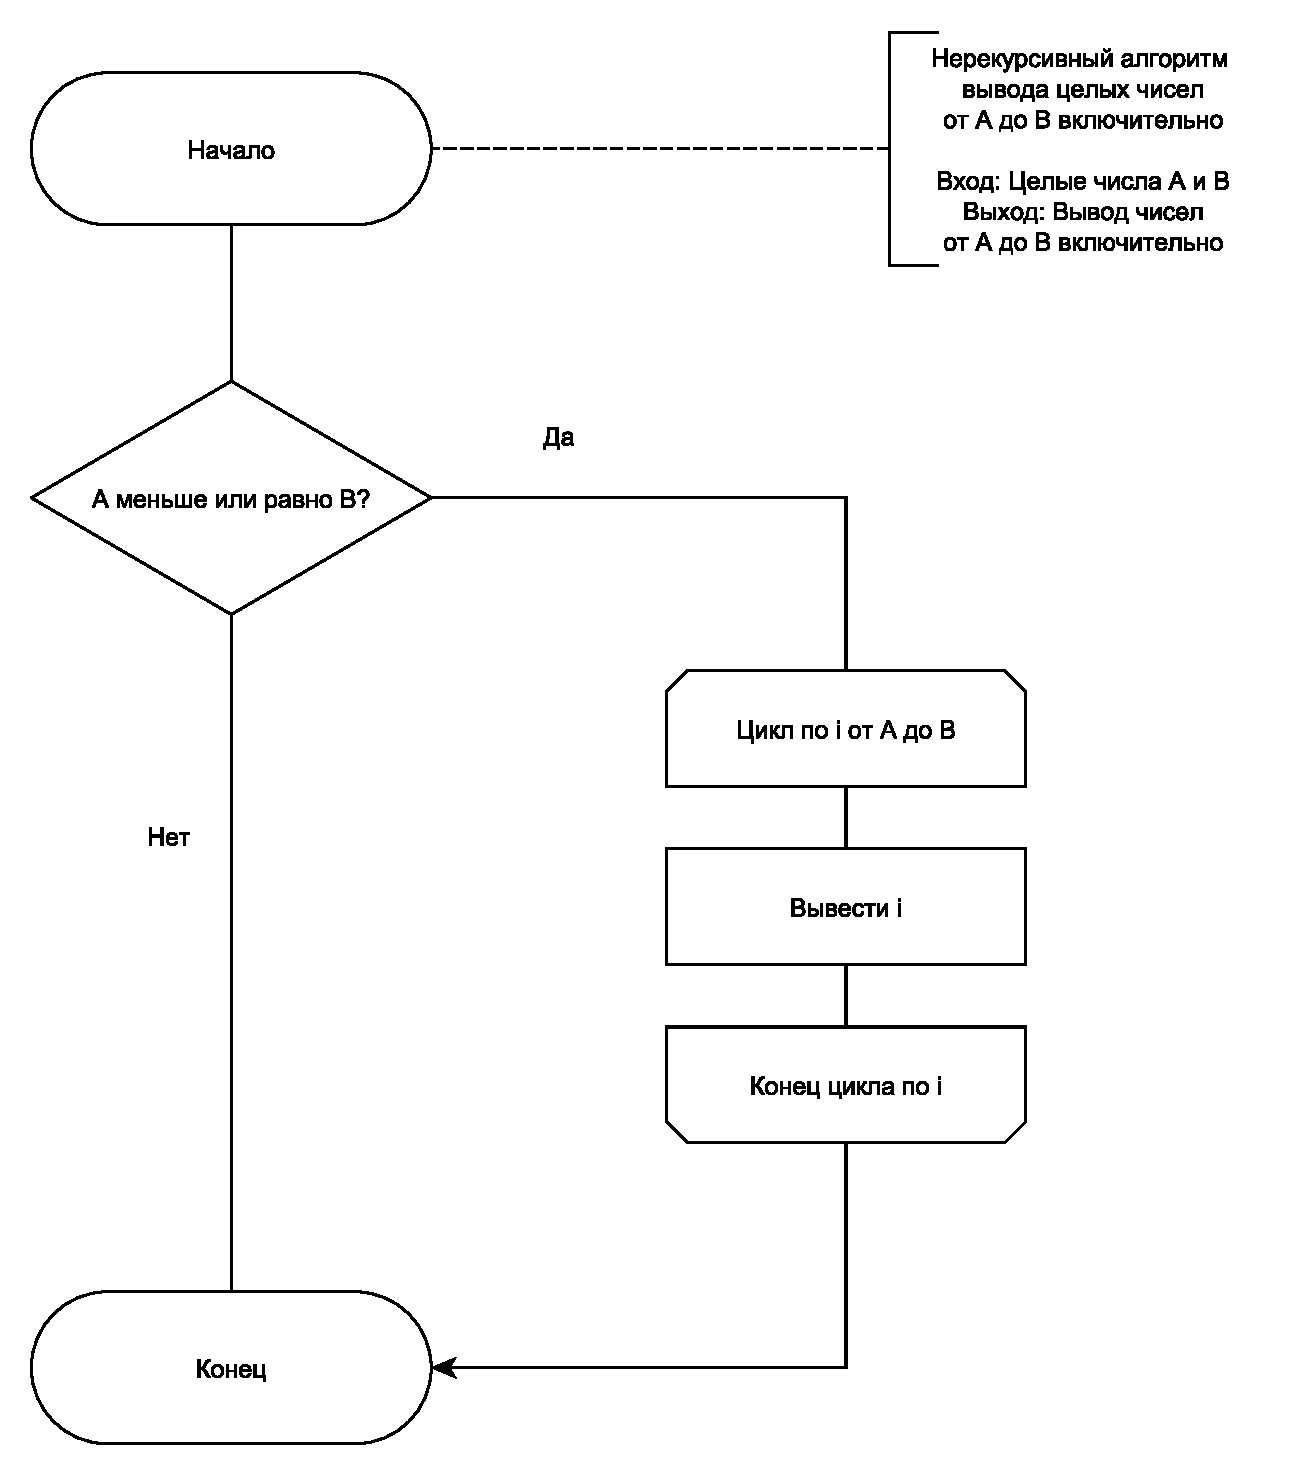
\includegraphics[width=0.8\textwidth]{images/shema_num1}
	\caption{Схема нерекурсивного алгоритма}
	\label{fig:shemanum1}
\end{figure}

\clearpage
\section{Рекурсивный алгоритм}

Схема алгоритма приведена на рисунке~\ref{fig:shemanum2}.  

\begin{figure}[h!]
	\centering
	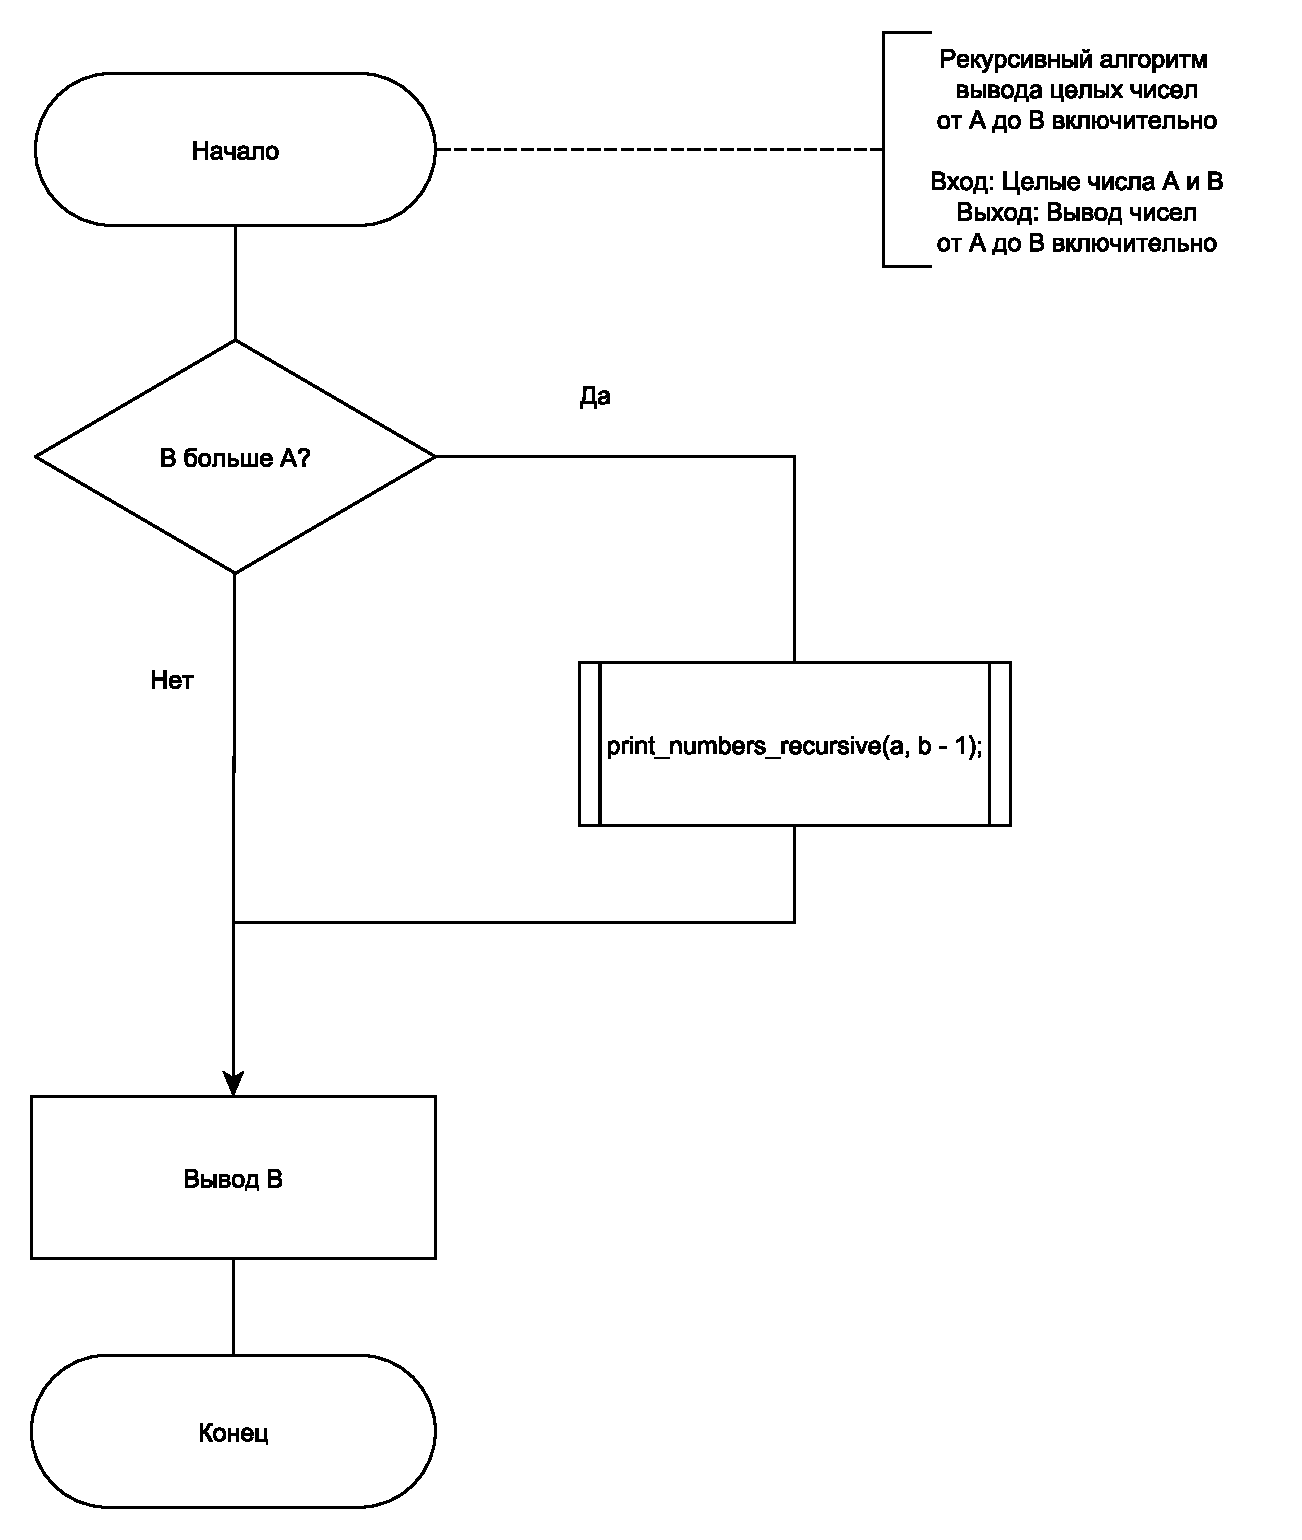
\includegraphics[width=0.8\textwidth]{images/shema_num2}
	\caption{Схема рекурсивного алгоритма}
	\label{fig:shemanum2}
\end{figure}

\clearpage

\section{Теоретическая оценка трудоёмкости и потребления памяти}

\subsection{Трудоёмкость нерекурсивного алгоритма}

Нерекурсивная реализация выполняет единственный вызов функции и цикл, проходящий по диапазону значений от $a$ до $b$.\\
Так как функция вызывается один раз, накладные расходы имеют постоянное значение:
\begin{equation}
	\label{eq:call_overhead}
	T_{\text{call}} = O(1)
\end{equation}
В теле функции выполняется цикл длиной $N$, где
\begin{equation}
	\label{eq:N_def}
	N = b - a + 1
\end{equation}
Каждая итерация включает служебные операции и операцию вывода. Пусть время одной итерации равно $(t_s + t_o)$, где $t_s$~--- стоимость служебных действий, а $t_o$~--- стоимость вывода числа. Тогда суммарная трудоёмкость цикла равна:
\begin{equation}
	\label{eq:iter_total}
	T_{\text{loop}}(N) = N \cdot (t_s + t_o)
\end{equation}
Общая трудоёмкость нерекурсивного алгоритма складывается из затрат на вызов функции~(\ref{eq:call_overhead}) и выполнения цикла~(\ref{eq:iter_total}):
\begin{equation}
	\label{eq:T_nonrec_total}
	T_{\text{nonrec}}(N) = T_{\text{call}} + T_{\text{loop}}(N)
\end{equation}
Подставляя выражения~(\ref{eq:call_overhead}) и~(\ref{eq:iter_total}), получаем:
\begin{equation}
	\label{eq:T_nonrec_asymp}
	T_{\text{nonrec}}(N) = O(1) + \Theta(N) = \Theta(N)
\end{equation}
Таким образом, асимптотическая оценка времени выполнения нерекурсивного алгоритма равна $\Theta(N)$, где $N = b - a + 1$~(\ref{eq:N_def}).

\subsection{Трудоёмкость рекурсивного алгоритма}

Для анализа рекурсивного варианта введём параметры:
\begin{equation}
	\label{eq:params_values}
	p = 2, \quad r = 3, \quad k = 0, \quad l = 0, \quad f = 1
\end{equation}
Память, выделяемая при каждом вызове функции, определяется как сумма параметров, локальных переменных, служебных регистров и одной дополнительной ячейки для хранения адреса возврата:
\begin{equation}
	\label{eq:frame_size}
	F = f + p + k + r + l + 1
\end{equation}
После подстановки значений из~(\ref{eq:params_values}) имеем:
\begin{equation}
	\label{eq:frame_numeric}
	F = 1 + 2 + 0 + 3 + 0 + 1 = 7
\end{equation}
Глубина рекурсии обозначается через $d$ и определяется числом последовательных вызовов:
\begin{equation}
	\label{eq:d_depth}
	d = b - a + 1
\end{equation}
Тогда общий объём используемой памяти вычисляется по формуле:
\begin{equation}
	\label{eq:stack_total}
	M_{\text{rec}} = F \cdot d
\end{equation}
С учётом~(\ref{eq:frame_numeric}) и~(\ref{eq:d_depth}):
\begin{equation}
	\label{eq:stack_subst}
	M_{\text{rec}} = 7 \cdot (b - a + 1)
\end{equation}
Асимптотически:
\begin{equation}
	\label{eq:M_rec_asymp}
	M_{\text{rec}} = \Theta(b - a + 1)
\end{equation}
Каждый рекурсивный вызов выполняет проверку условия, арифметические операции и вывод значения. Пусть:
\begin{align}
	\label{eq:f_leaf_def}
	f_{\text{leaf}} &= 1 + 2 = 3,\\
	\label{eq:f_internal_def}
	f_{\text{internal}} &= 1 + 1 + 2 = 4,\\
	\label{eq:f_overhead_def}
	f_{\text{overhead}} &= 2 \cdot F = 14
\end{align}
Тогда общее время работы алгоритма:
\begin{equation}
	\label{eq:total_time_rec}
	T_{\text{rec}} = d \cdot f_{\text{overhead}} + (d - 1) \cdot f_{\text{internal}} + f_{\text{leaf}}
\end{equation}
После упрощения~(\ref{eq:total_time_rec}) получаем:
\begin{equation}
	\label{eq:total_time_numeric}
	T_{\text{rec}}(d) = 18d - 1
\end{equation}
Подставляя значение глубины рекурсии из~(\ref{eq:d_depth}):
\begin{equation}
	\label{eq:T_rec_final}
	T_{\text{rec}}(b, a) = 18 \cdot (b - a + 1) - 1 = \Theta(b - a + 1)
\end{equation}

\section{Вывод}

Рекурсивный алгоритм имеет линейную временную сложность $T_{\text{rec}} = \Theta(b - a + 1)$ (см.~\ref{eq:T_rec_final}) и линейную оценку потребляемой памяти $M_{\text{rec}} = \Theta(b - a + 1)$ (см.~\ref{eq:M_rec_asymp}).
Таким образом, нерекурсивная реализация является более эффективной как по времени выполнения, так и по потреблению памяти.